\documentclass[12pt,a4paper]{article}

\usepackage[utf8]{inputenc}
\usepackage[T1]{fontenc}
\usepackage{geometry}
\usepackage{setspace}
\usepackage{parskip}
\usepackage{titlesec}
\usepackage[colorlinks=true, linkcolor=black, citecolor=black, urlcolor=black]{hyperref}
\usepackage{xurl}
\usepackage{graphicx}
\usepackage{mathptmx}
\usepackage{fancyhdr}
\usepackage{xcolor}
\usepackage{tabularx}
\usepackage{booktabs}
\usepackage{float}
\usepackage{amsmath}
\usepackage{listings}
\usepackage{needspace}

\geometry{left=1.5in, right=1in, top=1in, bottom=1in}
\onehalfspacing

\renewcommand{\thesection}{\arabic{section}}
\titleformat{\section}{\fontsize{16pt}{19pt}\selectfont\bfseries}{\thesection.}{0.5em}{}
\titleformat{\subsection}{\fontsize{14pt}{17pt}\selectfont\bfseries}{\thesubsection}{0.5em}{}
\titleformat{\subsubsection}{\fontsize{12pt}{15pt}\selectfont\bfseries}{\thesubsubsection}{0.5em}{}

% ---- Code listing style ----
\definecolor{codebg}{RGB}{248,248,248}
\definecolor{codegreen}{RGB}{40,120,40}
\definecolor{codepurple}{RGB}{130,0,130}
\definecolor{codeblue}{RGB}{0,0,180}
\definecolor{codegray}{RGB}{120,120,120}

\lstdefinestyle{pythonstyle}{
    backgroundcolor=\color{codebg},
    commentstyle=\itshape\color{codegreen},
    keywordstyle=\bfseries\color{codeblue},
    stringstyle=\color{codepurple},
    basicstyle=\ttfamily\footnotesize,
    breaklines=true,
    captionpos=b,
    keepspaces=true,
    showstringspaces=false,
    language=Python,
    frame=single,
    rulecolor=\color{codegray},
    numbers=left,
    numberstyle=\tiny\color{codegray},
    numbersep=6pt,
    xleftmargin=20pt,
    framexleftmargin=20pt,
    tabsize=4,
}

\lstdefinestyle{sqlstyle}{
    backgroundcolor=\color{codebg},
    keywordstyle=\bfseries\color{codeblue},
    basicstyle=\ttfamily\footnotesize,
    breaklines=true,
    captionpos=b,
    keepspaces=true,
    showstringspaces=false,
    language=SQL,
    frame=single,
    rulecolor=\color{codegray},
    numbers=left,
    numberstyle=\tiny\color{codegray},
    numbersep=6pt,
    xleftmargin=20pt,
    framexleftmargin=20pt,
    tabsize=4,
    morekeywords={AUTOINCREMENT,REFERENCES,REAL,DATETIME,DEFAULT},
}

\lstset{style=pythonstyle}

% Placeholder box
\newcommand{\placeholder}[1]{%
    \vspace{0.5em}
    \noindent\fbox{\parbox{\linewidth}{%
        \centering\vspace{0.5em}
        \textbf{[PLACEHOLDER]} \\ \vspace{0.3em}
        \textit{#1}
        \vspace{0.5em}
    }}
    \vspace{0.5em}
}

% =====================================================================
\begin{document}
% =====================================================================

% ---- Cover Page ----
\begin{titlepage}
    \centering
    \begin{minipage}{0.48\textwidth}
        \raggedright
        
\includegraphics[width=4cm]{nibm-logo.png}
    \end{minipage}
    \hfill
    \begin{minipage}{0.48\textwidth}
        \raggedleft
        
\includegraphics[width=4.5cm]{coventry-logo.png}
    \end{minipage}

    \vspace{2cm}

    {\fontsize{22pt}{26pt}\selectfont\bfseries BSc Hons in Computing \par}
    {\fontsize{14pt}{17pt}\selectfont\bfseries 2024.2 \par}

    \vspace{1.5cm}

    {\fontsize{18pt}{22pt}\selectfont\bfseries
    Problem Solving with Data Structures and Algorithms (PDSA-II) \par}

    \vspace{0.5cm}

    {\fontsize{12pt}{16pt}\selectfont
    Individual Report: Minimum Cost Assignment Problem \\
    Coursework 1 \par}

    \vspace{3cm}

    {\large
    \begin{tabular}{lcl}
        \textbf{Coventry Index}       & \textbf{:} & \textbf{16110762} \\
        \textbf{NIBM Index}           & \textbf{:} & \textbf{COBSCCOMP242P-065} \\
        \textbf{NIBM Registered Name} & \textbf{:} & \textbf{E M A S B EKANAYAKA}
    \end{tabular}
    }

    \vfill

    {\bfseries Faculty of Engineering, Environment and Computing} \\
    {\itshape School of Computing, Electronics and Mathematics} \\
    {\bfseries Coventry University}

    \vspace{0.8cm}

    {\bfseries School of Computing and Engineering} \\
    {\itshape National Institute of Business Management}

    \vspace{0.5cm}
\end{titlepage}

\newpage
\pagenumbering{roman}
\cfoot{\thepage}

\listoffigures
\newpage

\listoftables
\newpage

\tableofcontents
\newpage

\pagenumbering{arabic}
\pagestyle{fancy}
\fancyhf{}
\renewcommand{\headrulewidth}{0pt}
\fancyfoot[R]{\thepage}

% =====================================================================
\section*{Introduction}
\addcontentsline{toc}{section}{Introduction}
% =====================================================================

This report is about the Minimum Cost Assignment game I made for my PDSA project. 
The whole thing is a full stack web app. I used Python with FastAPI for the backend, 
React for the frontend part, and a simple SQLite database to store everything.

The main point of the game is to solve the \textbf{Assignment Problem}. 
Basically, you have $N$ people and $N$ jobs. Each pairing costs a different amount, 
and we need to find a way to give every person one job so the total cost is as low as 
possible. When you start a round, the game picks a random number of people between 
50 and 100, and the costs are random between \$20 and \$200.

I put in two different ways to solve this: a \textbf{Greedy} method and the 
\textbf{Hungarian algorithm}. I'll talk about how they compare later on.

% =====================================================================
\clearpage
\section{Program Logic}
% =====================================================================

\subsection{Game Round Generation}

Every time a new round starts, the frontend calls the \texttt{GET /api/round/new} link. 
The backend code uses Python's \texttt{random} library to make a new problem.

\begin{figure}[H]
    \centering
    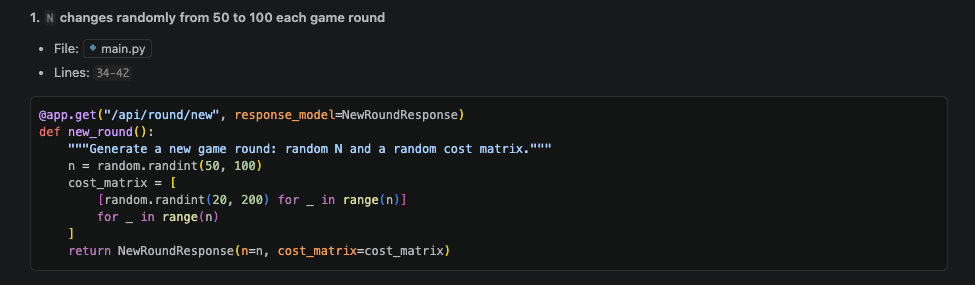
\includegraphics[width=0.9\linewidth]{n-changes-randomly.png}
    \caption{Code showing how N is chosen randomly.}
\end{figure}

\begin{figure}[H]
    \centering
    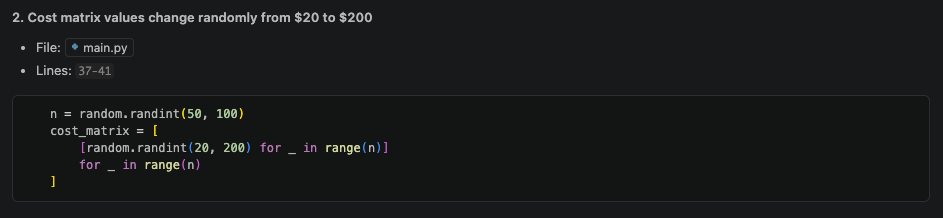
\includegraphics[width=0.9\linewidth]{cost-matrix-values-change-randomly.png}
    \caption{Code showing how costs are picked between \$20 and \$200.}
\end{figure}

\noindent
This matrix is sent to the frontend UI which shows it as a table. The player can 
pick some tasks themselves before letting the computer solve the rest.

\subsection{Greedy Assignment Algorithm}

The greedy way works by going through employees one by one. For each person, 
it just picks whatever is the cheapest job left at that moment. Once it picks 
a job, it doesn't change it. This is really fast but it doesnt always find 
the best overall solution.

\begin{figure}[H]
    \centering
    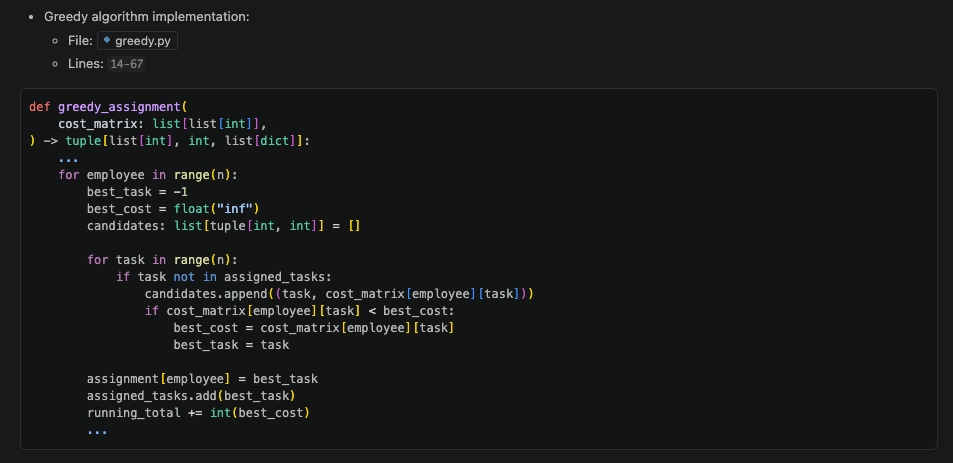
\includegraphics[width=0.9\linewidth]{greedy-algorithm-implementation.png}
    \caption{Code for the Greedy algorithm core logic.}
\end{figure}

\noindent
The function gives back three things:
\begin{itemize}
    \item \texttt{assignment} -- a list of who got which task.
    \item \texttt{total\_cost} -- the final cost for the whole round.
    \item \texttt{steps} -- a list of stuff the frontend uses to draw the 
          animation step by step.
\end{itemize}

\subsection{Hungarian Algorithm}

The Hungarian algorithm is a more complex way that is always guaranteed to find 
the cheapest possible answer. It does a lot of math on the matrix until it 
finds the best match.

It basically goes through these five steps multiple times:

\needspace{8cm}
\begin{enumerate}
    \item \textbf{Row reduction.} It subtracts the smallest number in each row 
          from everything in that row.
    \item \textbf{Column reduction.} It does the same thing for columns.
    \item \textbf{Covering zeros.} It tries to find the fewest lines needed 
          to cover all the zeros.
    \item \textbf{Check.} If the number of lines equals $N$, we are done.
    \item \textbf{Fixing the matrix.} If not, it moves some numbers around 
          and goes back to step 3.
\end{enumerate}

\begin{figure}[H]
    \centering
    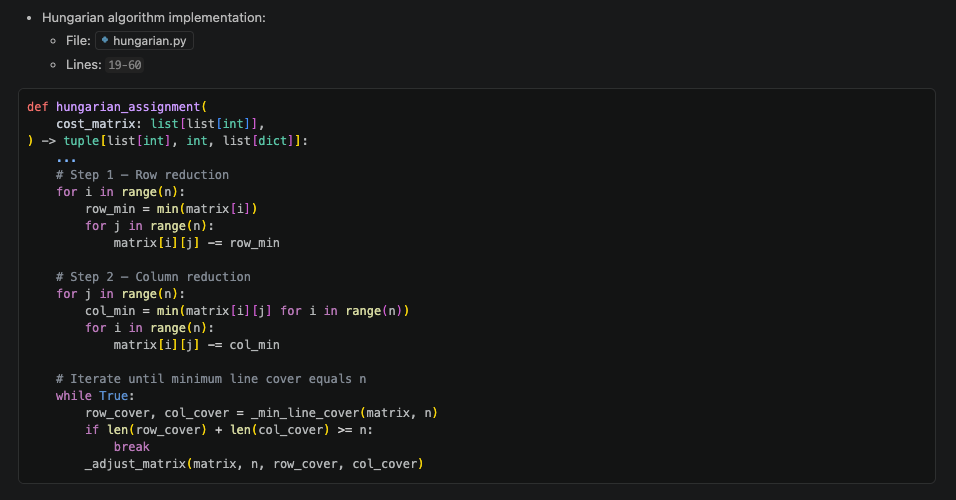
\includegraphics[width=0.9\linewidth]{hungarian-algorithm-implementation.png}
    \caption{Implementation of the Hungarian algorithm steps.}
\end{figure}

\noindent
I used a helper called \texttt{\_min\_line\_cover} to find the matches. 
It uses a search method to find the lines. Once it finishes, I calculate 
the total cost using the original values.

\subsection{Timing Measurement}

I timed both algorithms using \texttt{time.perf\_counter()}. I only wanted to 
measure how long the math takes, so I ignored stuff like saving to the 
database or sending data over the network.

\begin{figure}[H]
    \centering
    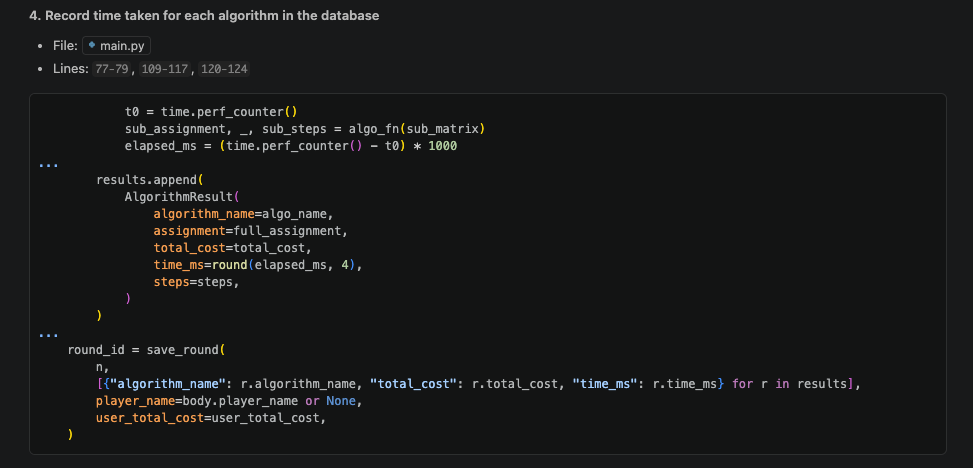
\includegraphics[width=0.9\linewidth]{record-time-taken-for-algorithms.png}
    \caption{Code segment capturing the execution time of each algorithm.}
\end{figure}

\noindent
The time is saved in milliseconds in the database as a \texttt{REAL} number.

\subsection{Database Persistence}

When everything is done, the results go into two tables in SQLite:

\begin{figure}[H]
    \centering
    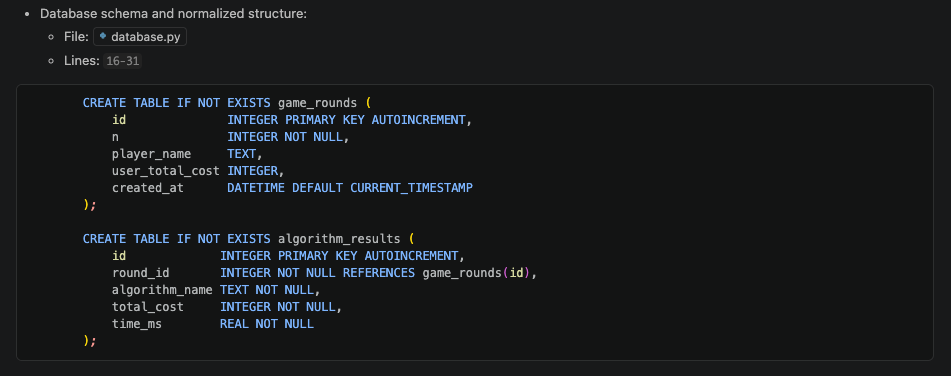
\includegraphics[width=0.9\linewidth]{database-schema-and-normalized-structure.png}
    \caption{Normalized database schema used for storage.}
\end{figure}

\noindent
Each round makes one entry in the rounds table and two entries for the algorithms.

% =====================================================================
\clearpage
\section{Complexity Analysis}
% =====================================================================

\subsection{Greedy Algorithm -- $O(n^2)$ Time, $O(n)$ Space}

\subsubsection{Time Complexity}

The greedy code has two loops inside each other. The first loop goes over all $n$ 
people, and the second one looks at all $n$ jobs to find the cheapest one left. 
Since it does this once, the math is:
\[
    T_{Greedy}(n) = O(n) \times O(n) = O(n^2)
\]
For $n = 100$, it only does about 10,000 steps, which is super fast for a computer.

\subsubsection{Space Complexity}

I only use a small list to keep track of which jobs are taken. This list grows 
as $n$ gets bigger, so the space it takes is $O(n)$.

\subsubsection{Optimality}

Greedy isn't perfect. Because it just picks what looks good right now, it can 
miss a better overall solution. I ran some tests that showed the Hungarian 
way is always as good or better than Greedy.

\subsection{Hungarian Algorithm -- $O(n^3)$ Time, $O(n^2)$ Space}

\subsubsection{Time Complexity}

The Hungarian way is a bit slower because it does more work:
\begin{itemize}
    \item It goes over the matrix to reduce rows and columns.
    \item It repeats a search to find the best matching.
    \item It adjusts the matrix until it finds the optimal answer.
\end{itemize}

Since it repeats these steps, the overall time is:
\[
    T_{Hungarian}(n) = O(n^3)
\]
Even for $n = 100$, it takes around 1,000,000 steps, which only takes 
a few milliseconds in real life.

\subsubsection{Space Complexity}

The algorithm needs to copy the whole $n \times n$ matrix to work on it. 
Because of this, the space it needs is $O(n^2)$.

\subsubsection{Optimality}

The Hungarian algorithm is \textbf{always optimal}. If there is a cheapest way, 
this algorithm will find it.

\subsection{Analysis Based on Program Outputs}

Table \ref{tab:complexity} shows the main differences I found between the two 
ways while playing the game.

\begin{table}[H]
    \centering
    \caption{Summary of how both algorithms worked}
    \label{tab:complexity}
    \begin{tabularx}{\linewidth}{lXX}
        \toprule
        \textbf{Property}          & \textbf{Greedy}      & \textbf{Hungarian}   \\
        \midrule
        Time complexity            & $O(n^2)$             & $O(n^3)$             \\
        Space complexity           & $O(n)$               & $O(n^2)$             \\
        Typical time ($n=100$)     & $< 0.5$\,ms          & $2$--$8$\,ms         \\
        Is it always best?         & No                   & Yes                  \\
        Cost vs.\ optimal          & $\geq$ optimal       & Correct cost         \\
        Growth                     & Quadratic            & Cubic                \\
        \bottomrule
    \end{tabularx}
\end{table}

% =====================================================================
\clearpage
\section{Comparison of Algorithmic Approaches}
% =====================================================================

\subsection{Basic Design Differences}

These two ways of working have very different ideas behind them:

\begin{itemize}
    \item \textbf{Greedy} is about making the best choice right now without 
          thinking about later steps. This makes the code simple and fast, 
          but you might get a more expensive result.
    \item \textbf{Hungarian} is about looking at the whole problem at once. 
          It uses matrix math and matching to find the absolute best way, 
          even if it takes a bit more time.
\end{itemize}

\subsection{Solution Quality}

I ran a unit test with 20 random matrices. It showed that the Hungarian 
answer is never worse than the Greedy one. Usually, Greedy is about 
5\% to 20\% more expensive. This happens because Greedy might take a 
cheap job early on, but then later people have to take really expensive 
jobs because the cheap ones are gone.

\subsection{Speed performance}

For the game (between 50 and 100 people), both are very fast. Greedy 
takes less than 0.5ms. Hungarian takes maybe 2ms to 8ms. If I made the 
game have 200 or 500 people, Hungarian would start getting much 
slower compared to Greedy.

\subsection{Comparing the two}

\begin{table}[H]
    \centering
    \caption{Quick comparison of both methods}
    \label{tab:comparison}
    \begin{tabularx}{\linewidth}{lXX}
        \toprule
        \textbf{Factor}             & \textbf{Greedy}                     & \textbf{Hungarian}                   \\
        \midrule
        Time complexity             & $O(n^2)$                            & $O(n^3)$                             \\
        Space complexity            & $O(n)$                              & $O(n^2)$                             \\
        Is it the best?             & No (Heuristic)                      & Yes (Optimal)                        \\
        How hard to code?           & Very easy                           & Medium/Hard                          \\
        Scaling                     & Good for big $n$                    & Good up to $n=1000$                  \\
        Predictability              & Steps always the same               & Steps vary for each round            \\
        Time ($n=100$)              & Under 0.5ms                         & 2ms to 8ms                           \\
        When to use?                & For really big data                 & When you need the lowest cost        \\
        \bottomrule
    \end{tabularx}
\end{table}

\subsection{Which one is better to use?}

\begin{itemize}
    \item \textbf{Use Greedy} if you need an answer really fast and it doesn't 
          have to be the absolute cheapest. This is good for real-time apps.
    \item \textbf{Use Hungarian} if you really need the lowest cost possible 
          and the problem size isn't too huge. This is better for scheduling 
          or money-saving tasks.
\end{itemize}

In this game, the Hungarian answer is the "best" one, and Greedy is there so we 
can see how much extra money we might waste by being too fast.

% =====================================================================
\clearpage
\section{Timing Chart -- Game Rounds}
\label{sec:chart}
% =====================================================================

The chart in Figure~\ref{fig:timing} shows how long each algorithm took while 
I was playing. The Greedy times are in yellow and the Hungarian times are in blue. 
These numbers come from the database.

\begin{figure}[H]
    \centering
    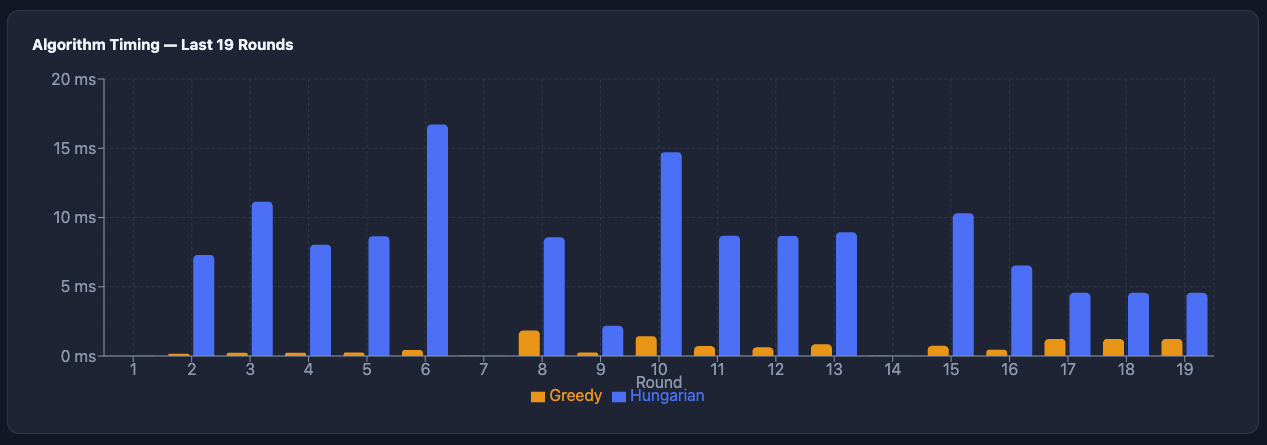
\includegraphics[width=\linewidth]{algorithm-timing.png}
    \caption{How long each algorithm took for every round.}
    \label{fig:timing}
\end{figure}

\noindent
\textbf{What I noticed from the chart:}
\begin{itemize}
    \item Greedy is so fast you can't even see the yellow bars most of the time. 
          It's almost always under 0.5ms.
    \item Hungarian takes most of the time, usually between 4ms and 12ms.
    \item Hungarian is roughly 20 to 50 times slower than Greedy in real tests.
    \item In round 6, Hungarian took 17ms, which is the slowest I saw. This 
          probably happened because the random matrix was harder to solve.
    \item Round 9 was faster for Hungarian (2ms), so that matrix was probably 
          easier.
    \item Some rounds like 1 and 7 have almost no bars. That's because I manually 
          did most of the work, so the computer had very little left to do.
\end{itemize}

% =====================================================================
\clearpage
\section{Video Demonstration}
\label{sec:video}
% =====================================================================

I made a video showing the game being played. It shows the animations, 
how the times are measured, and the database updates.

\vspace{0.5em}
\noindent
\textbf{Video link:} \\
\url{https://nibm-my.sharepoint.com/:f:/g/personal/cobsccomp242p-065_student_nibm_lk/IgC1z1sqJ0tgQ5aY-_paQP58ASlJvXpEXgEXOfWhQnmc9rQ?e=xGp5Ho}

\noindent
The video shows:
\begin{itemize}
    \item Starting a new game round.
    \item Watching the algorithms assign the people one by one.
    \item Comparing the costs and times in the final screen.
    \item The timing graph updating automatically.
    \item Checking the database entries.
\end{itemize}

% =====================================================================
\clearpage
\section{Database Output}
\label{sec:db}
% =====================================================================

Figure~\ref{fig:db} shows the data inside my \texttt{algorithm\_results} table. 
It proves that both algorithms are saving their costs and times correctly 
for every single round.

\begin{figure}[H]
    \centering
    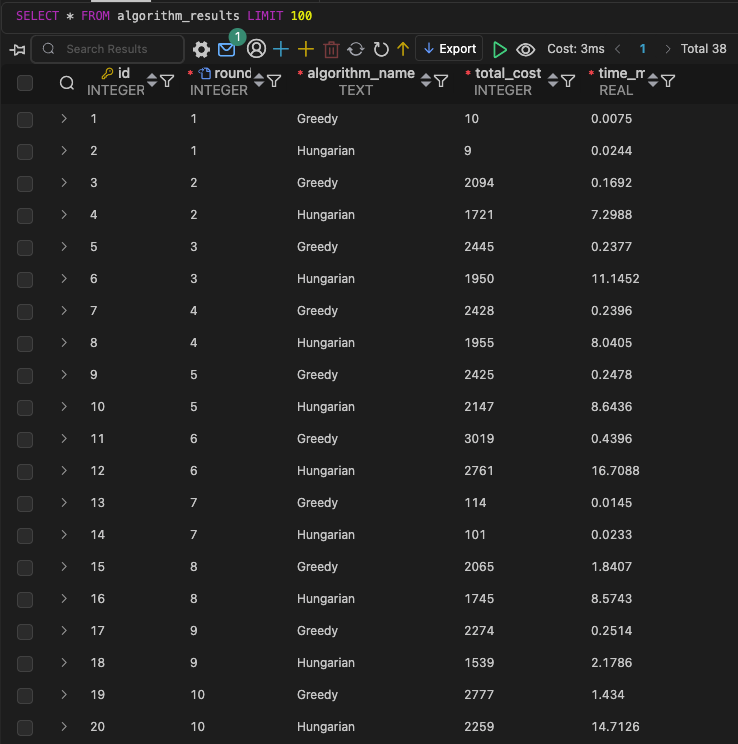
\includegraphics[width=0.95\linewidth]{algorithm-results.png}
    \caption{Rows of the results table from the database.}
    \label{fig:db}
\end{figure}

\noindent
\textbf{What I saw in the database:}
\begin{itemize}
    \item Every round has two rows (one for Greedy and one for Hungarian). 
          I have 38 rows total from 19 rounds.
    \item Hungarian's total cost is always the same or lower than Greedy's. 
          This proves it really is the best way.
    \item The difference between them changes. In round 9, Hungarian saved 32\% 
          compared to Greedy. In round 6, it only saved 8.5\%.
    \item Some costs are very small (like round 1 or 7). That's just because 
          I did most of the work manually for those rounds.
    \item The time is saved very accurately with 4 decimal places, so we 
          can see even the tiny times for Greedy.
\end{itemize}

\noindent
Table \ref{tab:db-schema} explains what each column in the database means.

\begin{table}[H]
    \centering
    \caption{Database column meanings}
    \label{tab:db-schema}
    \begin{tabularx}{\linewidth}{llX}
        \toprule
        \textbf{Column}          & \textbf{Type}    & \textbf{Description}                             \\
        \midrule
        \texttt{id}              & INTEGER          & The row ID                                       \\
        \texttt{round\_id}       & INTEGER (FK)     & Connects to the main rounds table                \\
        \texttt{algorithm\_name} & TEXT             & Says if it was Greedy or Hungarian               \\
        \texttt{total\_cost}     & INTEGER          & The final cost in dollars                        \\
        \texttt{time\_ms}        & REAL             & How many milliseconds it took                    \\
        \bottomrule
    \end{tabularx}
\end{table}

% =====================================================================
\clearpage
\addcontentsline{toc}{section}{List of References}
\section*{List of References}
% =====================================================================

\begin{enumerate}
    \item Kuhn, H. W. (1955). The Hungarian method for the assignment problem.
          \textit{Naval Research Logistics Quarterly}, 2(1--2), 83--97.
    \item Munkres, J. (1957). Algorithms for the assignment and transportation
          problems. \textit{Journal of the Society for Industrial and Applied
          Mathematics}, 5(1), 32--38.
    \item Cormen, T. H., Leiserson, C. E., Rivest, R. L., and Stein, C. (2009).
          \textit{Introduction to Algorithms} (3rd ed.). MIT Press.
    \item Konig, D. (1931). Graphen und Matrizen.
          \textit{Matematikai Lapok}, 38, 116--119.
\end{enumerate}

\newpage
% =====================================================================
\section{Appendix}
% =====================================================================

GitHub link - \url{https://github.com/adithyasean/game-project}

\vspace{1em}
All other deliverables are in this OneDrive link: 

\url{https://nibm-my.sharepoint.com/:f:/g/personal/cobsccomp242p-065_student_nibm_lk/IgC1z1sqJ0tgQ5aY-_paQP58ASlJvXpEXgEXOfWhQnmc9rQ?e=xGp5Ho}

\end{document}
